%Diese LaTeX-Vorlage f�r Praktikumsprotokolle in Form einer Ver�ffentlichung f�r das 
%F-Praktikum wurde erstellt von Andreas Nuber EP II, Uni W�rzburg.
%Es wurde das Koma-Skript verwendet und sollte somit installiert sein
%desweiteren sollten alle packages installiert sein, die mit \usepackage{} 
%eingebunden werden.
%Zum Testen dieser Vorlage wurde MikTex verwendet sowie TeXnicCenter als Editor
%beim Compilieren waren 0 Fehler, 1 Warnung und 3 zu volle/leere Boxen. Das ist ok :)

%F�r das Erstellen einfach den sinnfreien Text, der zum ausf�llen genommen wurde 
%ersetzen. Was sonst noch ver�ndert werden sollte steht in den Kommentaren!


\documentclass[a4paper,10pt,twocolumn]{scrartcl} %Koma-Skript-�quivalent zu "article"

\usepackage{german}            %macht deutsche �berschriften
\usepackage{amsmath}           %macht
\usepackage{amsfonts}          %       Mathe
\usepackage{amssymb}           %              m�chtiger
\usepackage{graphicx}          %erlaubt Graphiken einzubinden (.eps f�r dvi und ps sowie .jpg f�r pdf)
\usepackage[T1]{fontenc}       %Zeichenbelegung der verwendeten Schrift
\usepackage{ae}                %macht sch�neres �
\usepackage{typearea}	         %erm�glicht �nderung des Seitenspiegels
\usepackage{scrlayer-scrpage}          %erm�glicht �nderung der Kopf-/Fu�zeile
\usepackage{lastpage}          %l�sst auf die Seienanzahl zugreifen
\usepackage[margin=10pt,font=small,labelfont=bf]{caption} %macht die Bildbeschriftungen richtig

\renewcommand{\figurename}{Abb.}

\pagestyle{scrheadings}        %sagt Koma-Skript, dass selbstdefiniers Kopfzeilen verwendet werden
\typearea{16}                  %stellt Seitenspiegel ein
\columnsep25pt								 %definiert Breite zwischen den zwei Spalten von \twocolumns

\renewcommand{\pnumfont}{%     %�ndert die Schriftart der Seitennummerierung
\normalfont\rmfamily\slshape}  %�ndert die Schriftart der Seitennummerierung 



\begin{document}
\cfoot{\thepage /\pageref{LastPage}}     %macht die Seitennumerierung der Fom 2/5 (ausser auf der Titelseite)

\twocolumn[{\csname @twocolumnfalse\endcsname                %erlaubt "Abstrakt" �ber beide Spalten
\titlehead{                                                  %Kopfzeile
	\begin{tabular*}{\textwidth}[]{@{\extracolsep{\fill}}lr}   %Kopfzeile
	Betreuer: Der Betreuer & \today\\                          %Kopfzeile      hier den Betreuer eintragen!!!
	\end{tabular*}                                             %Kopfzeile
	}
\title{Messung der Ausbreitungsgeschwindigkeit von elektromagnetischen Wellen auf Kabeln}  %Titel der Versuchs
\author{Moritz Langer \and Hannes Winkler}                     %Namen der Studenten
\date{07.11.2025}                                                         %ben�tigt um automatisches Datum auszuschalten
\maketitle                                                      %erzeugt Titelseite
\vspace{-8ex}                                                   %verringert Abstand zur �berschrift
\begin{abstract}                                                %Beginn des Abstracts
\vspace{1em}
Versuchsdurchführung: 06. November 2025\\       %Datum �ndern!
Protokollabgabe: 01. März 2006                 %Datum �ndern!
\vspace{1em}
\end{abstract}
}]

\section{Einleitung}


\section{Theorie}

	\subsection{Wellenausbreitung auf Kabeln}

		\subsubsection{Wellenwiderstand}

			Bei der Untersuchung von Kabeln gibt es zwei charakteristische Größen:
			Die relative Induktivität   $L* = \frac{\text{Induktivität}}{\text{Längeneinheit}}$
			und die relative Kapazität $C* = \frac{\text{Kapazität}}{\text{Längeneinheit}}$. Über
			deren Zusammenhang mit der Spannung 

			\begin{displaymath}
				U_{\pm}(x,t) = \sqrt{\frac{L*}{C*}} \cdot I_{\pm}(x,t) = Z \cdot I_{\pm}(x,t)
			\end{displaymath}
	
			lässt sich analog zu dem Ohmschen Gesetz der Wellenwiderstand Z des Kabels definieren.
			Wichtig zu beachten ist, dass es sich nicht um ein ohmschen Widerstand mit Verlusten
			handelt, sondern um einen Wellenwiderstand welcher das Verhältnis zwischen
			Spannung und Strom in dem Kabel angibt.
		
		\subsubsection{Reflexion}

			Sobald das Signal das Kabelende erreicht, wird es reflektiert. Die Art bzw. das Maß
			der Reflexion hängt hierbei von dem Widerstand $R_v$ ab, welcher sich an dem Ende befindet.
			Dieses Maß nennt sich der Reflexionskoeffizient $\rho$ welcher definiert ist über 
			das Verhältnis zwischen der Amplitude der auslaufenden und der Amplitude dereinlaufenden 
			Welle und kann mithilfe des Ohmschen Gesetzes weiter vereinfacht werden als:

			\begin{displaymath}
				\rho = \frac{U_{-}(x,t)}{U_{+}(x,t)} = \frac{R_v - Z}{R_v + Z}
			\end{displaymath}

			Anhand dieser Formel lassen sich drei Spezialfälle des Reflexionskoeffizient erkennen:

			\begin{enumerate}
				\item Kurzschluss der Leitung: \\
						Das reflektierte Signal entspricht dem einlaufenden Signal mit entgegengesetztem
						Vorzeichen. Die Wellen löschen sich am Kabelende aus\\
						Es gilt: $R_v = 0 \Omega \Rightarrow \rho = -1 $
				\item Offenes Ende der Leitung: \\
						Das reflektiert Signal ist gleich dem einlaufenden Signal und diese 
						addieren sich. \\
						Es gilt: $R_v = \infty \Rightarrow \rho = 1 $
				\item Reflexionsfreier Abschluss:
						Durch richtige Wahl des Abschlusswiderstandes bleibt die Reflexion aus und 
						es gibt nur eine einlaufende Welle. \\
						Es gild $R_v = Z \Rightarrow \rho = 0 $
			\end{enumerate}

		
		\subsubsection{Mathematische Beschreibung einer Welle}


\section{Experiment}

\begin{figure}[htbp]                                 %So bindet man Graphiken ein
\begin{center}                                       %zentriert die Graphik
%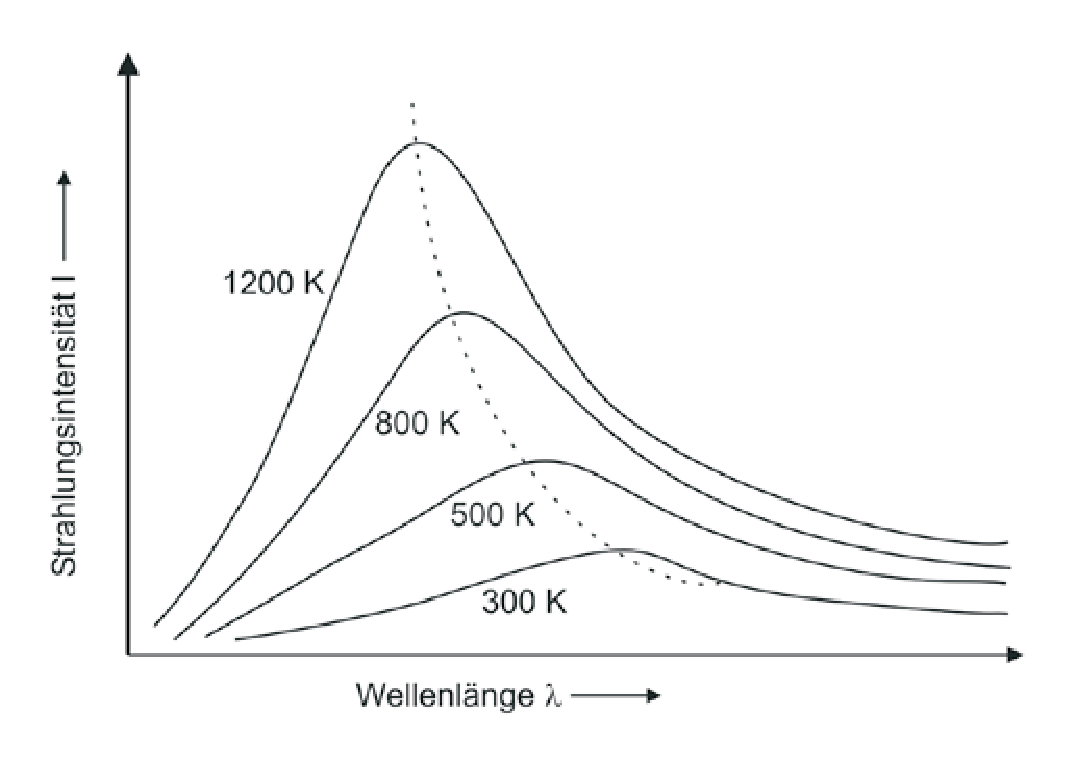
\includegraphics[width=0.9\linewidth]{bild1}       %das eingentliche Einbinden; "schwarz" ist der Dateiname ohne Endung
\caption[]{}   %Beschriftung der Graphik
\label{schwarz}                                      %das wird zu Zitiern im Text gebraucht
\end{center}
\end{figure}

\section{Auswertung}

\begin{table}[htbp]          %so funktionieren die Tabellen in LaTeX
\centering
\begin{tabular*}{\linewidth}{@{\extracolsep{\fill}}ccc}
\hline
\hline
\rule[-7pt]{0pt}{23pt}  Subshell  &     $j$ values 						  		&     Area ratio \\
\hline
\rule[-6pt]{0pt}{21pt}   $s$ 			&     $\frac{1}{2}$ 							&       --- \\

\rule[-6pt]{0pt}{21pt}   $p$ 			&     $\frac{1}{2},\frac{3}{2}$ 	&     $1:2$ \\

\rule[-6pt]{0pt}{21pt}   $d$ 			&     $\frac{3}{2},\frac{5}{2}$ 	&     $2:3$ \\

\rule[-7pt]{0pt}{22pt}   $f$ 			&     $\frac{5}{2},\frac{7}{2}$ 	&     $3:4$ \\
\hline
\hline
\end{tabular*}  
\caption[]{}  %siehe Graphik: Beschriftung
\label{spinsplit}                             %siehe Graphik: zum Zitieren
\end{table}

\section{Zusammenfassung}

\begin{thebibliography}{}    %so wird das Literaturverzeicnis erstellt
\bibitem{a}
\bibitem{b} 

\end{thebibliography}



\end{document}